\documentclass[10.5pt,a4paper]{ctexart}

\usepackage[top=16mm,bottom=16mm,left=18mm,right=18mm]{geometry}
\usepackage{fontspec}
\usepackage{graphicx}
\usepackage{enumitem}
\usepackage{xcolor}
\usepackage{hyperref}
\usepackage{qrcode}
\usepackage{microtype}
\usepackage{titlesec}

\setCJKmainfont{Songti SC}
\setCJKsansfont{PingFang SC}
\setmainfont{Helvetica Neue}
\setsansfont{Helvetica Neue}

\definecolor{navy}{HTML}{17324D}
\definecolor{ink}{HTML}{20242A}
\definecolor{muted}{HTML}{626A73}
\definecolor{rulegray}{HTML}{C7CDD3}

\hypersetup{
  hidelinks,
  pdfauthor={陈思翰},
  pdftitle={陈思翰 AdventureX 正式简历},
  pdfsubject={医学科研与 AI 产品经历}
}

\pagestyle{empty}
\setlength{\parindent}{0pt}
\setlength{\parskip}{0pt}
\color{ink}
\linespread{1.08}

\titleformat{\section}
  {\large\bfseries\sffamily\color{navy}}
  {}{0pt}{}
  [\vspace{2pt}{\color{rulegray}\titlerule[0.55pt]}]
\titlespacing*{\section}{0pt}{11pt}{6pt}

\setlist[itemize]{
  leftmargin=1.45em,
  label=\textcolor{navy}{\textbullet},
  itemsep=2.6pt,
  topsep=3pt,
  parsep=0pt,
  partopsep=0pt
}

\newcommand{\entry}[3]{%
  \textbf{#1}\hfill{\small\color{muted}#2}\\[-1pt]
  {\small\color{muted}#3}\par
}

\newcommand{\projectentry}[3]{%
  \textbf{#1}\hfill{\small\color{muted}#2}\\[-1pt]
  {\small\color{navy}#3}\par
}

\newcommand{\skillline}[2]{%
  \textbf{#1}\quad #2\par\vspace{2.5pt}
}

\begin{document}

\begin{minipage}[t]{0.79\textwidth}
  {\fontsize{23}{27}\selectfont\bfseries\sffamily 陈思翰}\\[3pt]
  {\large\sffamily\color{navy}口腔医学｜生物信息学｜AI 科研产品}\\[7pt]
  {\small
    广东广州 \quad | \quad
    +86 135-5988-7508 \quad | \quad
    \href{mailto:2683973782@qq.com}{2683973782@qq.com}\\[2pt]
    \href{https://github.com/cshinjnu-eng}{github.com/cshinjnu-eng} \quad | \quad
    \href{https://csh.bsbsanwu.xyz}{csh.bsbsanwu.xyz}
  }
\end{minipage}
\hfill
\begin{minipage}[t]{0.15\textwidth}
  \raggedleft
  \vspace{-4pt}
  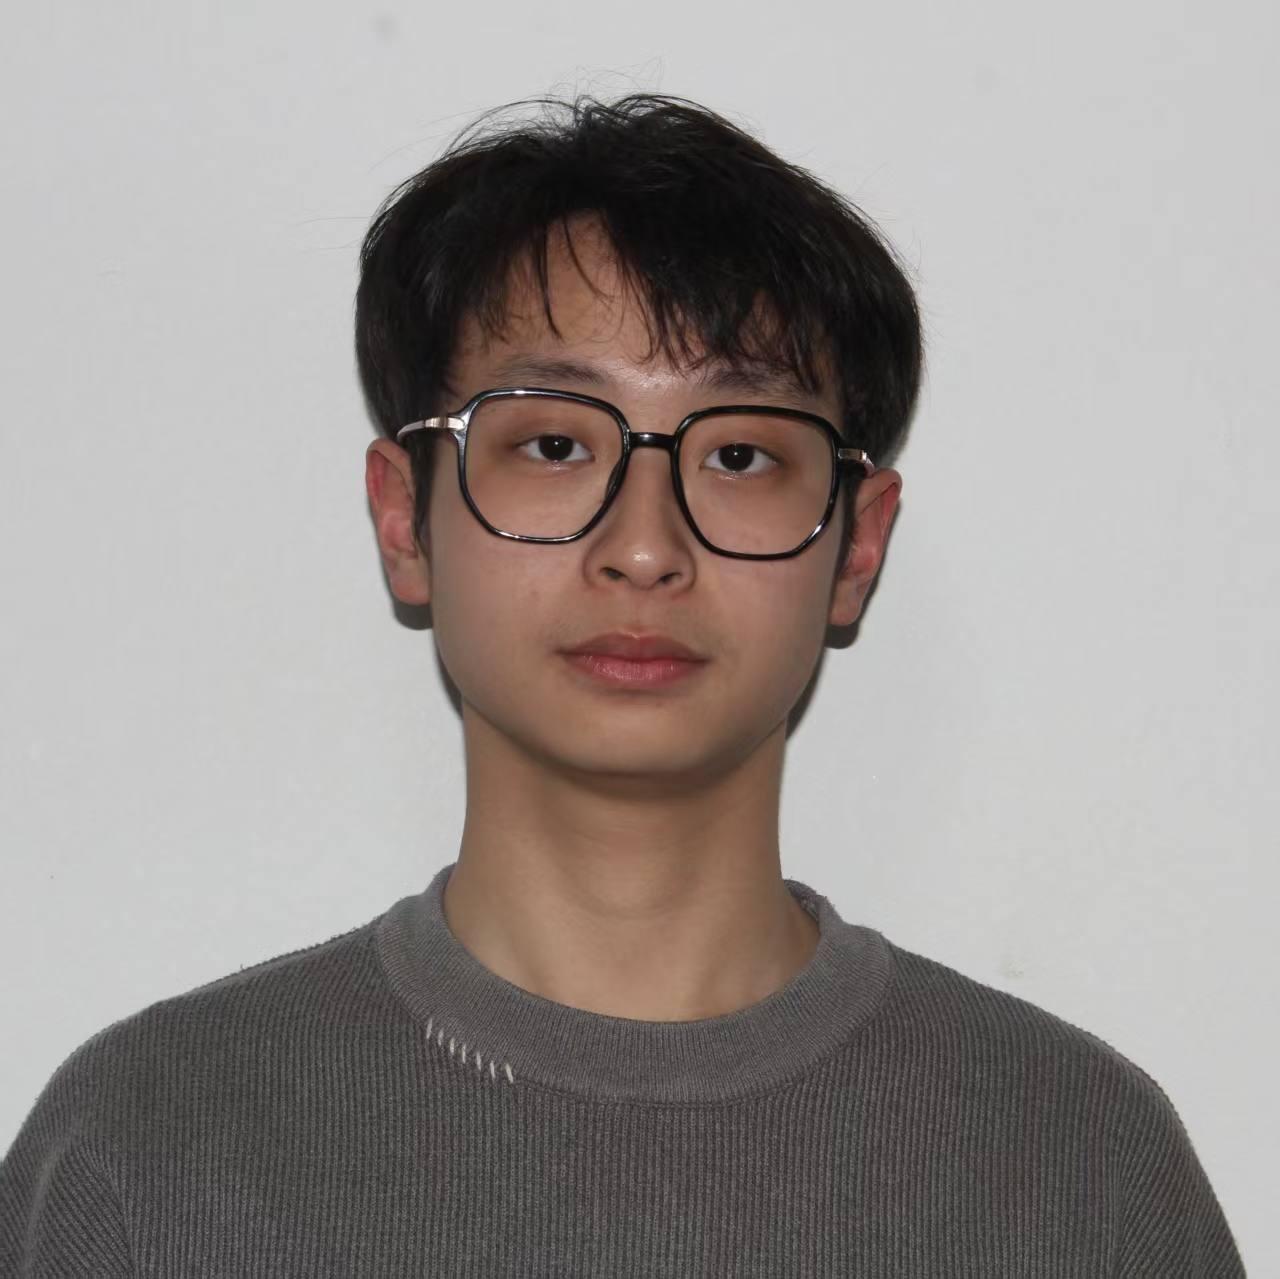
\includegraphics[width=23mm,height=30mm,keepaspectratio]{../assets/portrait.jpg}
\end{minipage}

\section{个人概述}

暨南大学 2025 级口腔医学学生，研究方向为 $\gamma\delta$T 细胞免疫衰老与单细胞生物信息学。能够从真实科研问题出发，独立完成数据分析、AI 工作流设计和全栈原型开发；希望继续参与科研 Agent 与单细胞分析工具的合作开发。

\section{教育背景}

\entry{暨南大学｜口腔医学}{2025 -- 至今}{本科在读｜广东广州}
\begin{itemize}
  \item 曾接受一年全英文临床医学培养，具备医学课程与英文专业资料学习基础。
\end{itemize}

\section{科研经历}

\entry{暨南大学基础医学与公共卫生学院｜研究助理、核心生信分析}{2024 -- 至今}{系统生物医学相关课题组}
\begin{itemize}
  \item 负责 $\gamma\delta$T 细胞多组学解析与免疫衰老跨器官异质性研究，从原始数据处理推进至投稿图表与结果解释。
  \item 独立完成 scRNA-seq 与 scTCR-seq 分析流程，包括质量控制、批次校正、聚类注释、细胞通讯、轨迹推断和可视化。
  \item 维护研究服务器、分析环境与项目文件；作为负责人推进 2 个科研项目，并参与免疫学实验方案设计。
  \item 目前有 3 篇 SCI 论文在投，持续参与研究结果复核、图表整理与投稿材料准备。
\end{itemize}

\section{核心项目}

\projectentry{scrna-omics｜单细胞分析 Agent 工作流}{2026 -- 至今}{独立设计与开发}
\begin{itemize}
  \item 面向单细胞分析中的方法选择、阶段确认、图表复核与决策记录，设计配置驱动的多智能体工作流。
  \item 将文献检索、代码生成、服务器执行、结果解释和生物学复核拆分为可追溯步骤，并用确定性 Hooks 管理关键质量门。
  \item 已在 2 个真实研究项目中使用，支持从分析计划到图表交付的连续工作；关键决策保留人工确认与审计记录。
  \item 项目演示：\href{https://scrna-omics.bsbsanwu.xyz/}{scrna-omics.bsbsanwu.xyz}
\end{itemize}

\vfill
{\footnotesize\color{muted}陈思翰｜AdventureX 2026 申请简历}\hfill{\footnotesize\color{muted}1 / 2}

\newpage

\begin{minipage}[t]{0.82\textwidth}
  {\fontsize{18}{22}\selectfont\bfseries\sffamily 陈思翰}\\[2pt]
  {\small\color{muted}产品开发、团队协作与综合能力}
\end{minipage}
\hfill
\begin{minipage}[t]{0.12\textwidth}
  \raggedleft
  \qrcode[height=14mm]{https://csh.bsbsanwu.xyz}\\[-1pt]
  {\scriptsize\color{muted}个人网站}
\end{minipage}

\section{产品与团队经历}

\projectentry{TimeBox｜时间管理与成长记录产品}{2026 -- 至今}{独立设计与开发｜Android、Web、AI Agent}
\begin{itemize}
  \item 将并行计时、待办、长线任务与成长记录组织在同一产品中；设计 Hermes 交互，用于补录遗漏、回顾当日进展和整理长期记录。
  \item 负责需求定义、交互设计、前后端实现和模型接入；项目入围粤港澳大湾区创新创业基地。
\end{itemize}

\projectentry{镜子｜多智能体观点调查与报告系统}{2026}{独立设计与开发｜Research Agent、报告自动化}
\begin{itemize}
  \item 将一句调研问题拆分为跨平台检索、信源分级、事实核查、质量检查和报告组装，形成 3 套报告系统。
  \item 为模板、格式和降级链建立 36 项自动化测试；代表报告：\href{https://mirror-opinion.bsbsanwu.xyz/r/degree/}{mirror-opinion.bsbsanwu.xyz/r/degree/}
\end{itemize}

\projectentry{GoGoWork｜任务协作平台}{2026 -- 至今}{创业团队核心成员｜产品与 PC 端开发}
\begin{itemize}
  \item 参与任务发布、人才匹配、资金托管和交付验收流程设计，并承担 PC 端原型与界面开发。
  \item 在团队环境中参与需求讨论、功能取舍和版本交付，积累跨角色协作与产品落地经验。
\end{itemize}

\section{内容与社群运营}

\entry{小红书账号“本硕博三无”｜内容策划与运营}{2026 -- 至今}{AI 咨询、医学科研辅助与产品分享}
\begin{itemize}
  \item 围绕生信实践、AI 工具、产品迭代与职业探索进行选题、写作和视频制作，并同步运营 2 个近 500 人的微信社群。
  \item 截至 2026 年 7 月，账号公开发布 24 条笔记和 4 条视频，累计近 5,000 次收藏与点赞。
\end{itemize}

\section{专利、荣誉与项目立项}

\entry{国家发明专利（已授权）｜基于人工智能的生物医学大数据分类方法及系统}{2025}{主要发明人之一｜授权公告号 CN120524301B｜申请号 CN202511016189.8}
\vspace{3pt}

\entry{全国大学生生命科学竞赛｜国家级三等奖}{2025}{第二成员}
\vspace{3pt}
\entry{暨南大学 AI+ 创新大赛｜三等奖}{2025}{校级竞赛}
\vspace{3pt}
\entry{暨南大学 AI+ 创新大赛｜二等奖}{2026}{校级竞赛}
\vspace{3pt}
\entry{校级创新创业项目｜2025 级立项}{2025 -- 至今}{项目负责人}

\section{技术能力}

\skillline{科研}{scRNA-seq、scTCR-seq、多组学生信分析、免疫学实验设计、文献计量与知识库构建}
\skillline{开发}{R、Python、JavaScript、全栈 Web、Android、后端架构、Linux 研究服务器}
\skillline{AI}{多智能体工作流、Hooks 与质量门、长期记忆、工具调用、模型接入与路由}
\skillline{产品}{用户调研、需求定义、原型验证、UI 与交互、内容生产、社群运营}
\skillline{语言}{中文；英文（曾接受一年全英文临床医学培养）}

\vfill
{\footnotesize\color{muted}陈思翰｜AdventureX 2026 申请简历}\hfill{\footnotesize\color{muted}2 / 2}

\end{document}
